\documentclass[../main/main.tex]{subfiles}


\begin{document}

\section{March 4th, 2021}
\subsection{Advanced Iterative Methods I}
In this chapter, we will develop non-stationary iterative methods. We will first do this using the projection method, and then improve it by incorporating preconditioning. Throughout this chapter, we assume $Ax=b$, where $A$ is SPD.
\subsubsection{Projection Methods with SPD Matrices}
Recall that for projection methods, the problem is reformulated as: Given $x_{0}$, generate $\tilde{x}$ by: \[
\begin{cases}
  \text{Find} &\tilde{x} \in  x_{0} +K \\
  \text{s.t.} & b - A\tilde{x} \perp L
\end{cases}
\]
In other words, we are finding

In matrix terms,
\begin{itemize}
\item Let $V = \begin{bmatrix}
v_1 & v_2 & \ldots  & v_{m}
\end{bmatrix} \in \RR ^{n\times m}$ be a basis of $K$
\item Let $W = \begin{bmatrix}
w_1 & w_2 & \ldots  & w_{m}
\end{bmatrix} \in \RR ^{n\times m}$ be a basis of $L$
\end{itemize}
Then: \[
\tilde{x} \in  x_{0} + K \implies  \tilde{x} = x_{0} + Vy \text{ for some $y\in \RR ^{m}$}
\] and\[
\]
\begin{align*}
  b-A\tilde{x} \perp L &\implies  \langle b-A(x_{0}+Vy), Wz\rangle = 0 \quad\forall z \in \RR ^{m}\\
                       &\iff  W^{T}(b-A(x_{0}+Vy)) = 0\\
  &\iff W^{T}AV y = W^{T}(Ax_{0}-b)
  .\end{align*}
This means that each step, we only need to solve the system of linear equations: $W^{T}AV y = W^{T}(Ax_{0}-b)$. Note that $W^{T}AV\in \RR ^{m\times m}$ which is smaller than $n$. \\

In order to preserve the structure of $A$ (SPD-ness), we choose $K=L$ (so that $W=V$). Then, we need to solve: \[
V^{T}AV y = V^{T} (Ax_{0}-b)
\]
\begin{remark}
Note that $V^{T}AV$ is SPD because $A$ is.
\end{remark}
\begin{theorem}
  $\tilde{x}$ is optimal in the sense that: \[
\tilde{x} = \operatorname{argmin}_{x\in x_{0}+K} \|x-x_{*}\|_{A}^2
  \] where $x_{*}$ is the true solution of $Ax=b$ and $\|\cdot \|_{A}$ is defined by $\|x\|_{A} = (x^{T}Ax)^{1 / 2}$.
\end{theorem}

In other words, if we project $x_{*}$ into the subspace, then the resulting $\tilde{x}$ is the closest point.

\begin{proof}
  Note that:

  \begin{align*}
    &\tilde{x} = \operatorname{argmin}_{x\in x_{0}+K} \|x-x_{*}\|_{A}^2 \\
    \iff & \langle x_{*} - \tilde{x}, (x_{0}+z) - \tilde{x} \rangle_{A} = 0 \quad  \forall  z \in K\\
    \iff & \langle A(x_{*}-\tilde{x}), (x_{0}+z)-\tilde{x}\rangle = 0 \quad  \forall  z \in  K\\
    \iff & \langle b-A\tilde{x}, (x_{0}-\tilde{x}) + z\rangle = 0 \quad  \forall  z \in  K
    .\end{align*}
  Since  $\tilde{x}$ satisfies: \[
\begin{cases}
  \tilde{x} \in  x_{0} + K \implies x_{0}-\tilde{x} \in  K \\
  \langle b-A\tilde{x},z\rangle = 0 \quad \forall  z \in  K
\end{cases}
\] \[
 \implies  \langle b-A\tilde{x}, (x_{0}-\tilde{x})+z\rangle = 0 \quad  \forall z \in  K
\]
\end{proof}
If we let $P_{K}^{(A)}$ denote the projection onto $K$ with $\|\cdot \|_{A}$, projection methods can be expressed as: \[
x_{k+1} = P_{x_{k}+K}^{(A)}(x_{*}), \quad  k=0,1,2, \ldots
\]
Note that this means that error is non-increasing under $A$-norm, as: \[
\|x_{k+1}-x_{*}\|_{A}\leq \|x_{K}-x_{*}\|_{A}
\]
However, this does not guarantee that the error converges to zero.

\subsubsection{One-Dimensional Projection Methods}
Now the question is how to choose $K$? In Gauss-Seidel, we choose the simplest one, i.e. $e_{i}$. \\

Given $x_{k}$, we choose $K$  s.t. $\text{dim}(K)=1$, i.e.: \[
K = \operatorname{span}\{d_{k}\}, \text{ where }d_{k} \in \RR ^{n}.
\]
\begin{remark}
 $d_{k}$ can be thought up as the direction.
\end{remark}
Now we might ask what is the best $d_{k}$? We have: \[
x_{k+1} = x_{k} + \alpha _{k}d_{k} \text{ for some } \alpha_{k} \in \RR
\]Assume we have fixed $\alpha_{k}\geq  0 $ and $\|d_{k}\|_{A}=\beta $. We want $\|x_{k+1}- x_{*}\|_{A}^2$ minimized. This gives us: \[
\]
\begin{align*}
  \|x_{k+1} - x_{*}\|_{A}^2 &= \|(x_{k}+\alpha_{k}d_{k}) - x_{*}\|^2_{A} \\
  &= \| x_{k}- x_{*}\|^2_{A} + \alpha _{k}^2 \|d_{k}\|^2_{A} + 2\alpha _{k}\langle d_{k}, x_{k}-x_{*}\rangle_{A}
  .\end{align*}
Note that $\| x_{k}- x_{*}\|^2_{A}$ and $\alpha _{k}^2 \|d_{k}\|^2_{A}$ are constants, meaning that in order to minimize the error, we want: \[
\min_{d_{k}\in \RR ^{n}}  \langle d_{k}, x_{k}-x_{*}\rangle_{A}
\]
Note that the solution to this is: \[
d_{k} = -C (x_{k}-x_{*})
\] where $C = \frac{\beta}{\|x_{k}-x_{*}\|_{A}} >0$.
\begin{remark}
The optimal $d_{k}$ is in the opposite direction of $x_{k}-x_{*}$.
\end{remark}
Finally, we choose: \[
K = \operatorname{span}\{d_{k}\} = \text{span}\{x_{k}-x_{*}\}
\]
However, we need to know $x_{*}$, which is not possible to know (since that is our goal). Thus this method is non-practical.
\begin{remark}
This is optimal only if we fixed $\|d_{k}\|_{A}$.
\end{remark}

Now let's consider fixing $\alpha _{k}\gtrsim 0$ and $\|d_{k}\|_{2}=\beta $.
\begin{remark}
 $\alpha _{k}\gtrsim 0$ means that it is greater but approximately zero.
\end{remark}
Again, we minimize $\|x_{k+1}-x_{*}\|_{2}^2$. Now we have:
\begin{align*}
  \|x_{k+1} - x_{*}\|_{A}^2 &= \|(x_{k}+\alpha_{k}d_{k}) - x_{*}\|^2_{A} \\
  &= \| x_{k}- x_{*}\|^2_{A} + \alpha _{k}^2 \|d_{k}\|^2_{A} + 2\alpha _{k}\langle d_{k}, x_{k}-x_{*}\rangle_{A}
  &\approx 2\alpha _{k}\langle d_{k}, x_{k}-x_{*}\rangle_{A} \quad (\text{since }\alpha_{k}\approx 0)
  .\end{align*}
Since $\alpha_{k}$ is a constant, we have:
\begin{align*}
 & \min _{\|d_{k}\|_{2}=\beta } \langle d_{k}, x_{k}- x_{*}\rangle_{A} \\
\iff  & \min_{\|d_{k}\|_{2}=\beta }  \langle d_{k}, Ax_{k}-b\rangle
  .\end{align*}
\begin{remark}
Note that the 2-norm ball is an ellipsoid in $\RR ^{n}$ with A-norm, thus, we change it to use the standard inner product. After doing this, the optimal $d_{k}$ is in the opposite direction of $Ax_{k}-b$.
\end{remark}
The solution to this equation is: \[
  d_{k} = -C(Ax_{k}-b)
\]where $c= \frac{\beta }{\|Ax_{k}-b\|_{2}}>0 $. Thus, the optimal choice of $K$ is: \[
K = \sspan \{d_{k}\} = \sspan \{r_{k}\}, \quad \text{where }r_{k} = b-Ax_{k}
\]
\begin{figure}[h!]
  \centering
  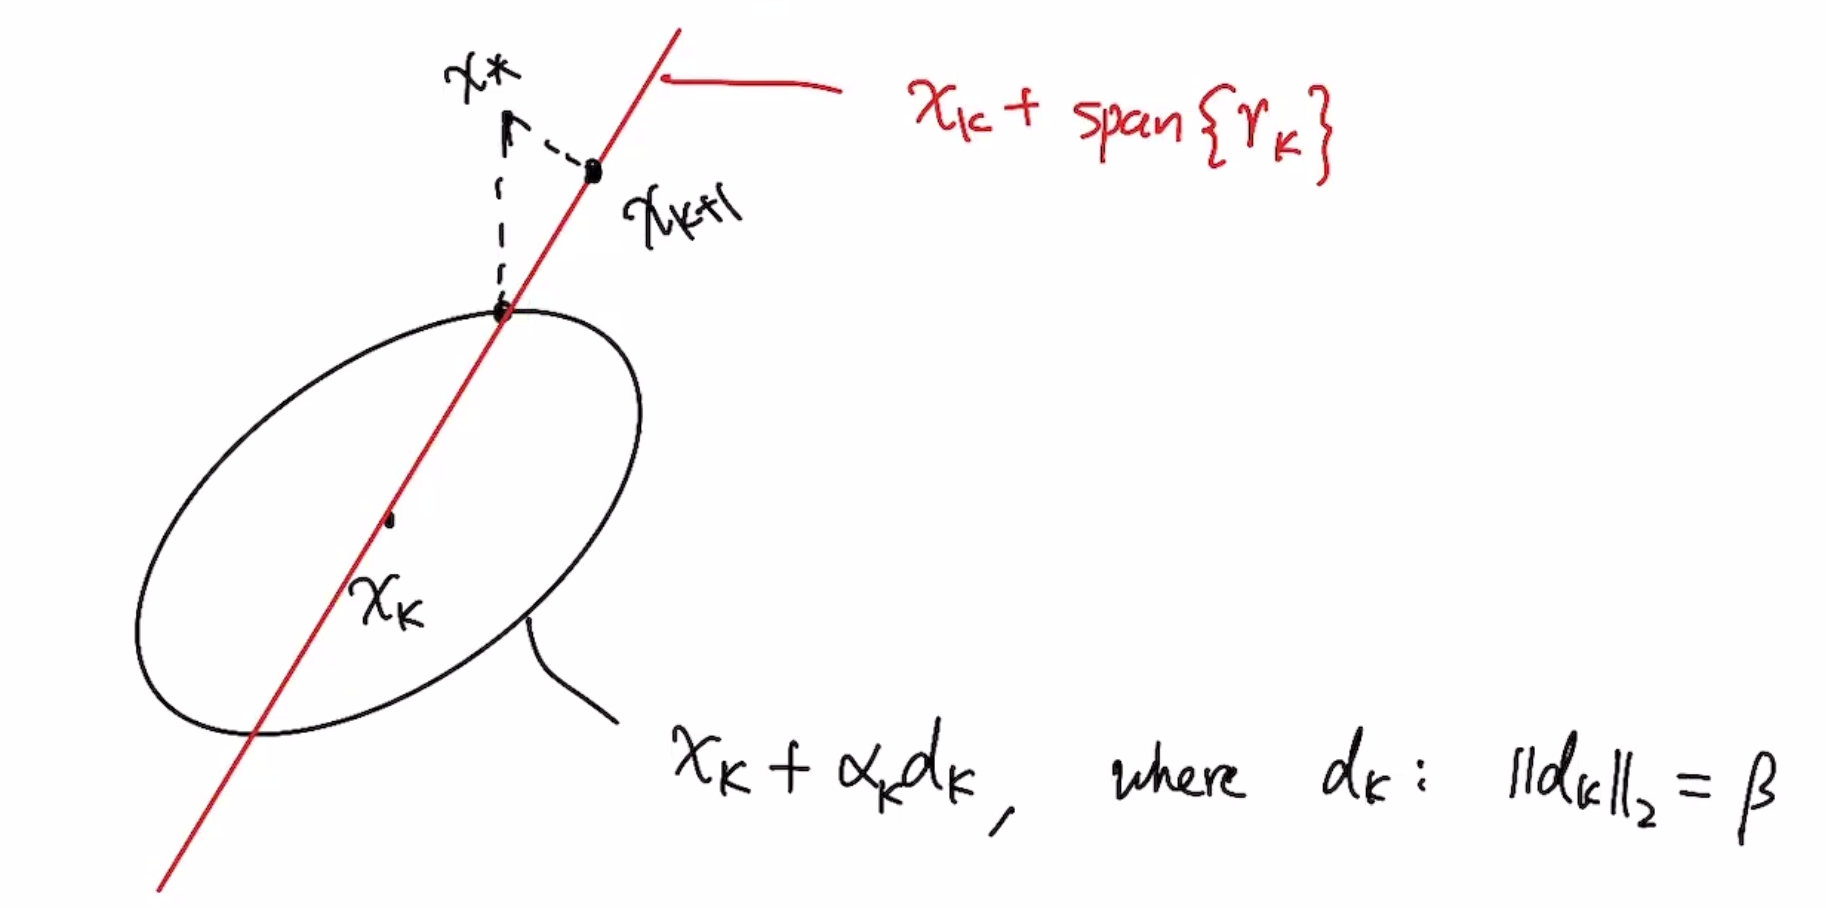
\includegraphics[width=0.8\textwidth]{../images/3-4-proj}
  \caption{Pictorial Version of $K$}
\end{figure}
Now we have found the optimal $K$, but the next step is to find the optimal $\alpha _{k}$.\\

In other words:
\begin{align*}
 & \min _{\alpha } \|(x_{k}+\alpha r_{k})-x_{*}\|_{A}^2\\
 \iff & \min _{\alpha }\|(x_{k}-x_{*})\|^2_{A}+ \alpha ^2 \|r_{k}\|_{A}^2 + 2\alpha \langle r_{k}, x_{k}-x_{*}\rangle_{A}
  .\end{align*}
Takign derivative w.r.t. $\alpha $ and setting it to 0, we have:
\begin{align*}
&  2\alpha \|r_{k}\|_{A}^2 + 2\langle r_{k}, x_{k}-x_{*}\rangle_{A}=0
                 \iff & \alpha = - \frac{\langle r_{k}, x_{k}- x_{*}\rangle_{A}}{\|r_{k}\|_{A}^2} =  - \frac{\langle r_{k}, Ax_{k}- b\rangle}{\|r_{k}\|_{A}^2}  = \frac{\|r_{k}\|_{2}^2}{\|r_{k}\|_{A}^2}
  .\end{align*}
Thus the optimal 1D projection method is given in Algorithm \ref{3-4-alg}.
        \begin{algorithm}[h!]
	\caption{Optimal 1D Projection Method}
    \label{3-4-alg}
	\begin{algorithmic}[1]
      \For{ $k=0,1,2, \ldots$}
 \State $r_{k}=b-Ax_{k}$
 \State $\alpha _{k} = \|r_{k}\|^2_{2} / \|r_{k}\|_{A}^2 = \frac{\iprod{r_{k}}{r_{k}}}{\iprod{Ar_{k}}{r_{k}}} $
 \State $x_{k+1} = x_{k}+\alpha _{k}x_{k}$
      \EndFor
	\end{algorithmic}
	\end{algorithm}
  \begin{remark}
Note that for each iteration, we use 2 matrix-vector products and $O(n)$ operations.
  \end{remark}
  This can be improved to 1 matrix-vector product. If we have denote $p_{k} = Ar_{k}$, then:
  \begin{align*}
    r_{k+1} &= b - Ax_{k+1} \\
            &= b-A(x_{k}+\alpha_{k}r_{l}) \\
            &= b-Ax_{k}-\alpha _{k}Ar_{k}\\
    = r_{k} - \alpha _{k} p_{k}
    .\end{align*}
  This gives us Algorithm \ref{3-4-alg2}.
        \begin{algorithm}[h!]
	\caption{Optimal 1D Projection Method Improved}
    \label{3-4-alg}
	\begin{algorithmic}[1]
      \State $r_{0}=b-Ax_{0}$
      \For{ $k=0,1,2, \ldots$}
      \State $p_{k} = Ar_{k}$
 \State $\alpha _{k} = \frac{\iprod{r_{k}}{r_{k}}}{\iprod{p_{k}}{r_{k}}} $
 \State $x_{k+1} = x_{k}+\alpha _{k}x_{k}$
 \State $r_{k+1} = r_{k}- \alpha _{k}p_{k}$
      \EndFor
	\end{algorithmic}
	\end{algorithm}
    Note that this is the algorithm Gradient descent for: \[
\min_{x\in \RR ^{n}} \frac{1}{2} x^{T}Ax-x^{T}b
\] with the exact line search, i.e.: \[
x_{k+1} = x_{k} -\alpha _{k}\nabla f(x_{k})
\] where $\alpha _{k} = \argmin_{\alpha  \in \RR } f(x_{k}-\alpha \nabla f(x_{k}))$. Thus, the algorithm is called: \vocab{steepest descent}.\index{steepest descent}
\end{document}
